\chapter{Machine Learning}
\nocite{Nilsson96introductionto}Si intende, per ML, una tecnica utilizzabile per risolvere problemi  nei quali si è in grado di specificare degli output dati determinati input senza però essere in grado di comprendere la relazione esistente tra i valori. Spesso problemi del tipo appena descritto portano con se un quantitativo di dati decisamente troppo vasto per essere analizzato soltanto da una o più persone, questa particolare tecnica offre dunque un modo più efficiente per svolgere analisi sui dati e rendere automatici determinati procedimenti consentendo anche di diminuire errori di tipo casuale dati dall'uomo, o addirittura catturare più informazioni rispetto a un operatore umano.\\
Il ML possiede un dominio di applicazione molto ampio, che può andare dalla medicina alla psicologia, e proprio per questo motivo esistono vari approcci e modalità. Nel mio lavoro di tirocinio in particolare è stato usato un approccio supervisionato.\\

\section{Apprendimento supervisionato}
Lo scopo di questo sistema è come dice la parola stessa, di supervisionare una macchina, questo costruendo un \emph{data-set}  \footnote{Il data-set è un insieme di dati raccolti da misurazioni svolte in fase di preparazione per lo studio del problema, classificati in modo opportuno.}
di valori, solitamente dei tipi che seguono: numerici, che devono essere normalizzati \footnote{Per normalizzazione si intende un processo che rende paragonabili dati tra loro di diversa natura fornendo valori compresi tra 0 e 1, ciò ottenuto nel modo seguente:\newline $\forall x_{i}, i\subset\mathbb{N}$ $x_{norm} = \dfrac{x_{i}-x_{min}}{x_{max} - x_{min}} $} prima di essere usati, nominali, stringhe oppure date, che serviranno come punto di riferimento alla macchina per costruire le regole che permetteranno di restituire precisi output dati determinati input.\\
Il ML con apprendimento supervisionato si divide in problemi di classificazione o di regressione. Il Caso in questione rientra nel tipo di classificazione, dunque un problema che dato un valore, o insieme di valori, restituisce un risultato discreto appoggiandosi a un \emph{albero di decisione} (DT) che la macchina ha costruito a partire da un meta-algoritmo, ciò dopo essere stata allenata con i dati di interesse.\\

\section{Alberi di decisione} 
Un albero di decisione è una tecnica di ML supervisionato, questo si divide in due tipologie: di classificazione e di regressione.
Un DT di classificazione permette di classificare i dati in modo discreto, le sue variabili infatti sono delle categorie come possono essere maschio e femmina, giallo e rosso e via dicendo.
Un DT di regressione viene usato per restituire delle predizioni dati dei valori di input, solitamente appartenenti all'insieme dei reali.\\
Come il nome suggerisce sono delle strutture ad albero dove ogni nodo in base a un valore consente di continuare in una direzione piuttosto che un'altra fino ad arrivare al termine di questo albero e dunque della decisione, termine che si trova nei nodi foglia, ovvero quelli finali.
%Un albero di decisione è una tecnica di ML supervisionato, i cui nodi interni sono dei test sui valori forniti, e el foglie sono le categorie a cui possono appartenere i valori di input \cite{Nilsson96introductionto}.
Questa struttura decisionale viene costruita tramite dei \emph{meta-algoritmi}\footnote{Ovvero si tratta di un algoritmo che non risolve il problema, ma è in grado di costruire lui stesso un nuovo algoritmo.} ad esempio J48, usato nel nostro caso, un'estensione del suo predecessore ID3 che prevede i seguenti passaggi:
\newpage
\begin{enumerate}
	\item Iterazione di ogni attributo su cui avviene il calcolo dell'\emph{entropia}, o, valore compreso tra 0 e 1.
	\item Selezione dell'attributo con l'entropia\footnote{Misura che indica la quantità di incertezza di un valore, misurabile nel modo che segue $E\left(X\right) = \sum_{x\in X} -p\left(x\right)log_{2}p(x)$ con $S$ il data-set su cui si vuole calcolare l'entropia, $X$ il set di classi in $S$ e in fine $p\left(x\right)$ il numero di elementi di classe $x$ nel set $S$} minore.
	\item Divisione (split)\footnote{Il data-set su cui vengono svolti i calcoli, viene diviso in due a partire dall'attributo con una minor entropia. Ciò porterà ad avere il primo sub-set conterrà tutte le istanze che avranno un determinato valore della classe osservata, il secondo possederà invece tutte le tuple contenenti il valore altro dell'attributo, se si ha un terzo valore che può assumere l'attributo si avrà un terzo sub-set, e così via per tanti quanti sono i valori possibili che questo può assumere.} del data-set sull'attributo con minore entropia.
\end{enumerate}
I passaggi appena descritti sono la sintesi del seguente pseudocodice:

\begin{algorithm}
	\begin{algorithmic}
		\Procedure{ID3}{$Esempi$, $AttributoTarget$, $Attributi$}
			\State Crea un nodo $Radice$.
			\If{Se tutti gli esempi sono positivi}
				\State restituisci un albero con un unico nodo $Radice$ ed etichetta = +
			\ElsIf{Se tutti gli esempi sono negativi}
				\State restituisci un albero con un unico nodo $Radice$ ed etichetta = -
			\ElsIf{Se Attributi è vuoto}
				\State restituisci un albero con un unico nodo $Radice$ ed etichetta = il valore di $AttributoTarget$ più comune tra le istanze di Esempi.
			\Else
				\State $A \leftarrow $ L'elemento di Attributi che riduce maggiormente l'entropia.
				\ForAll{$v$ in $A$}
					\State Aggiungi un nuovo ramo sotto $Radice$ corrispondente al test $A = v$.
					\State $Esempi(i) \leftarrow$ sottoinsieme di $Esempi$ che hanno valore $v$ per $A$.
					\If{$Esempi$ è vuoto}
						Aggiungi una foglia con etichetta = valore $AttributoTarget$ più comune tra gli esempi.
					\Else
						\State Aggiungi sotto $Radice$ il sottoalbero ID3 ($Esempi(v)$, $AttributoTarget$, $Attributi$ – ${A}$).
					\EndIf
				\EndFor
			\EndIf
		\EndProcedure
	\end{algorithmic}
%	ID3 (Examples, Target_Attribute, Attributes)
%	Create a root node for the tree
%	If all examples are positive, Return the single-node tree Root, with label = +.
%	If all examples are negative, Return the single-node tree Root, with label = -.
%	If number of predicting attributes is empty, then Return the single node tree Root,
%	with label = most common value of the target attribute in the examples.
%	Otherwise Begin
%	A ← The Attribute that best classifies examples.
%	Decision Tree attribute for Root = A.
%	For each possible value, vi, of A,
%	Add a new tree branch below Root, corresponding to the test A = vi.
%	Let Examples(vi) be the subset of examples that have the value vi for A
%	If Examples(vi) is empty
%	Then below this new branch add a leaf node with label = most common target value in the examples
%	Else below this new branch add the subtree ID3 (Examples(vi), Target_Attribute, Attributes – {A})
%	End
%	Return Root
\end{algorithm}

Questi passaggi teoricamente andrebbero ripetuti per ogni sub-set fino a ottenerne di puri\footnote{Dove ogni uno di essi contiene una sola sola tupla}, operazione però non sempre possibile per le dimensioni spesso molto grandi dei set di dati. Vengono dunque presi in esame vari fattori come la dimensione del data-set, o il livello di precisione accettabile per interrompere l'esecuzione dell'algoritmo. Un altro caso possibile di interruzione si ha nel momento in cui viene calcolata un'entropia pari a 1.\\

Per comprendere meglio è possibile considerare il seguente data-set che consentirà di decidere se una partita può o meno essere giocata in base alle condizioni meteorologiche.

\begin{table}[h!]
	\begin{center}
		\begin{tabular}{l|c|c|c|r} % <-- Alignments: 1st column left, 2nd middle and 3rd right, with vertical lines in between
			\textbf{Tempo} & \textbf{Temperatura} & \textbf{Umidità} & \textbf{Vento} & \textbf{Si Gioca}\\
			%			$\alpha$ & $\beta$ & $\gamma$ \\
			\hline
			sole     & caldo  & alta    & no & no \\
			sole     & caldo  & alta    & si & no \\
			nuvoloso & caldo  & alta    & no & si \\
			pioggia  & media  & normale & no & si \\
			pioggia  & freddo & normale & no & si \\
			pioggia  & freddo & normale & si & no \\
			nuvoloso & freddo & normale & si & no \\
			sole     & media  & alta    & no & no \\
			sole     & freddo & normale & no & si \\
			pioggia  & media  & normale & no & si \\
			sole     & media  & normale & si & si \\
			nuvoloso & media  & alta    & si & si 
		\end{tabular}
		\caption{Data-set di esempio iniziale.}
		\label{tab:data-set-example_1}
	\end{center}
\end{table}

Si procede dunque calcolando l'entropia per il data-set con 7 esiti positivi e 5 negativi il risultato risulterà la seguente informazione:\\ $I\left(D\right) = E\left(\frac{7}{12}; \frac{5}{12}\right) = -\left(\frac{7}{12} log_2\left(\frac{7}{12} \right) +  \frac{5}{12} log_2\left(\frac{5}{12} \right)\right) = 0.98$
\\Ora è possibile calcolare l'entropia dei singoli attributi.\\
Si osserva il tempo su tutto il set per cominciare\\
$I(tempo, D) = \frac{|D(tempo=sole)|}{|D|} +  \frac{|D(tempo=pioggia)|}{|D|} + \frac{|D(tempo=nuvoloso)|}{|D|}\\ 
= \frac{5}{12} I(D(tempo=sole)) + \frac{4}{12} I(D(tempo=pioggia)) + \frac{3}{12} I(D(tempo=nuvoloso))\\ 
= \frac{5}{12} E\left(\frac{2}{5};\frac{3}{5}\right) + \frac{4}{12} E\left(\frac{3}{4};\frac{1}{4}\right) + \frac{3}{12} E\left(\frac{2}{3};\frac{1}{3}\right) = 0.74$\\
Questo procedimento andrà eseguito per ogni attributo, quindi temperatura, umidità e vento ancora. Se vengono svolti i calcoli per i restanti si avrà che il l'entropia minore si ha proprio per la temperatura, risulteranno dunque i seguenti data-set:

\begin{table}[h!]
	\begin{center}
		\begin{tabular}{l|c|c|c|r} % <-- Alignments: 1st column left, 2nd middle and 3rd right, with vertical lines in between
			\textbf{Tempo} & \textbf{Temperatura} & \textbf{Umidità} & \textbf{Vento} & \textbf{Si Gioca}\\
			%			$\alpha$ & $\beta$ & $\gamma$ \\
			\hline
			sole     & caldo  & alta    & no & no \\
			sole     & caldo  & alta    & si & no \\
			sole     & media  & alta    & no & no \\
			sole     & freddo & normale & no & si \\
			sole     & media  & normale & si & si
		\end{tabular}
		\caption{caption.}
		\label{tab:data-set-example_2}
		
		\begin{tabular}{l|c|c|c|r} % <-- Alignments: 1st column left, 2nd middle and 3rd right, with vertical lines in between
			\textbf{Tempo} & \textbf{Temperatura} & \textbf{Umidità} & \textbf{Vento} & \textbf{Si Gioca}\\
			%			$\alpha$ & $\beta$ & $\gamma$ \\
			\hline
			pioggia  & media  & normale & no & si \\
			pioggia  & freddo & normale & no & si \\
			pioggia  & freddo & normale & si & no \\
			pioggia  & media  & normale & no & si \\
		\end{tabular}
		\caption{caption.}
		\label{tab:data-set-example_3}
		
		\begin{tabular}{l|c|c|c|r} % <-- Alignments: 1st column left, 2nd middle and 3rd right, with vertical lines in between
			\textbf{Tempo} & \textbf{Temperatura} & \textbf{Umidità} & \textbf{Vento} & \textbf{Si Gioca}\\
			%			$\alpha$ & $\beta$ & $\gamma$ \\
			\hline
			nuvoloso & caldo  & alta    & no & si \\
			nuvoloso & freddo & normale & si & no \\
			nuvoloso & media  & alta    & si & si \\
		\end{tabular}
		\caption{caption.}
		\label{tab:data-set-example_4}
		
	\end{center}
\end{table}

uno con tutti tutti i valori dell'attributo tempo pari a ``sole'', uno con ``pioggia'', e uno con ``nuvoloso'' generando così la prima porzione di albero\ref{figure:DT_start}, la sua radice che presenterà 3 possibili percorsi, 1 per ogni tipo di meteo. A questo punto bisognerà ripetere i passaggi per ogni set che è stato ottenuto e fino a che ogni set sia puro.

\begin{figure}
	\begin{center}
		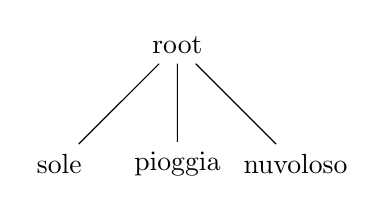
\begin{tikzpicture}
		\node(0){root}
		child{node{sole}}
		child{node{pioggia}}
		child{node{nuvoloso}};
		\end{tikzpicture}
	\end{center}
\caption{DT per il data-set di esempio}
\label{figure:DT_start}
\end{figure}

\section{I passaggi necessari}
Per costruire un sistema di classificazione intelligente con l'utilizzo del ML supervisionato, precisamente con weka sono dunque necessari vari passaggi. Il primo passaggio è la creazione di un data-set, questo potrà essere fatto in diversi modi, nel caso corrente il risultato è un file \href{https://www.cs.waikato.ac.nz/ml/weka/arff.html}{ARFF}\footnote{File di tipo testuale che presenta due sezioni, header e data. In header viene specificata la struttura e il tipo di dati per ogni tupla. In data vengono riportate le misurazioni o valori ordinati come specificato in header con i rispettivi valori.} contenente le features\footnote{Sono le caratteristiche di interesse del fenomeno che deve essere studiato} dei file audio che sono stati etichettati con le rispettive classi.\\
Segue poi una fase di allenamento dove viene costruito l'albero di decisione con un meta-algoritmo che può variare in base alle diverse esigenze e al tipo di problema in analisi. Generato il modello di classificazione creato ci si può comportare poi in diversi modi e decidere se validare o meno il risultato ottenuto, scegliendo dunque tra \emph{full train}, \emph{cross validation}, e \emph{training più test}. Scegliendo di lavorare in modalità full train si decide non effettuare validazioni rischiando così l'overfitting\footnote{Condizione per la quale un classificatore ha imparato a riconoscere casi troppo specifici e ha difficoltà in quelli più generali. Solitamente dato da un allenamento con una durata maggiore di quella necessaria oppure un data-set troppo piccolo.}. Per ridurre questo rischio è possibile dunque ricorrere a una tecnica di validazione come la modalità training più test andando così a dividere il data-set in due ottenendo così un sottoinsieme per il training e uno per il test, metodologia principalmente utilizzata con un elevato quantitativo di dati. Se per il problema che si intende risolvere la numerosità non è sufficiente per ottenere buoni risultati con la tecnica appena riportata, può allora essere considerata la metodologia di tipo cross validation consistente nella divisione del data-set in $k$ sottoinsiemi, $k-1$ di questi verranno utilizzati per l'allenamento e $1$ invece per il testing, operazione ripetuta $k$ volte.\\
Il classificatore che è stato ottenuto dovrà essere poi valutato per le sue capacità di classificare in modo corretto, passo generalmente svolto appoggiandosi a una \emph{matrice di confusione} (CM), questa fornirà delle informazioni riguardo ai valori che sono i \emph{true positive} (TP), \emph{true negative} (TN), \emph{false positive} (FP), \emph{false negative} (FN) e quindi comprendere le performances dell'algoritmo. Ogni sua colonna rappresenta i valori predetti, mentre e righe i valori reali.\\
Data la CM sarà possibile poi calcolare la \label{formula:accuracy}\emph{accuracy} come $ACC = \frac{TP+TN}{TP+TN+FP+FN}$, oppure \label{formula:sensitivity}\emph{sensitivity}) e \label{formula:specificity}\emph{specificity} dette anche \emph{true positive rate} (TPR) e \emph{true negative rate} (TNR), nei seguenti modi: $TPR = \frac{TP}{P}$  e $TNR = \frac{TN}{N}$.
%, in questo particolare caso è stato usato per classificare inizialmente \emph{nota} o \emph{non-nota}, dati dei campioni audio. Questo  evoluto per restituire 5 classi che indicano differenti gradi di essere nota o meno\footnote{La classe 5 significa essere certamente una nota, la classe 1 rappresenta invece una non nota, tutti i valori di mezzo rappresentano i diversi gradi tra l'essere nota o meno}.
